
\documentclass{article} % For LaTeX2e
\usepackage{iclr2026_conference,times}

% Optional math commands from https://github.com/goodfeli/dlbook_notation.
\input{math_commands.tex}

\usepackage{hyperref}
\hypersetup{colorlinks=true,linkcolor=blue,citecolor=blue,urlcolor=blue}
\usepackage{url}
\usepackage{amsmath,amssymb,amsthm}
\usepackage{algorithm}
\usepackage{algorithmic}
\usepackage{graphicx}
\usepackage{tikz}
\usetikzlibrary{calc}
\usepackage{booktabs}
\usepackage{subcaption}
\usepackage{enumitem}
\usepackage{bbm}

\newtheorem{theorem}{Theorem}
\newtheorem{lemma}[theorem]{Lemma}
\newtheorem{proposition}[theorem]{Proposition}
\newtheorem{corollary}[theorem]{Corollary}
\newtheorem{definition}{Definition}
\newtheorem{remark}{Remark}
\newtheorem{assumption}{Assumption}
\newtheorem{example}{Example}
\newtheorem*{theorem*}{Theorem}
\newtheorem*{lemma*}{Lemma}
\newtheorem*{proposition*}{Proposition}
\newtheorem*{corollary*}{Corollary}
\newtheorem*{remark*}{Remark}
\newcommand{\zz}[1]{\textcolor{blue}{(zz: #1)}}  
\newcommand{\hl}[1]{\textcolor{red}{#1}}  

\title{Beyond Best-of-Infinity:\\ Finite-Generation Limits of Test-Time LLM Ensembles}

% Authors must not appear in the submitted version. They should be hidden
% as long as the \iclrfinalcopy macro remains commented out below.
% Non-anonymous submissions will be rejected without review.

\author{Anonymous Authors}

% The \author macro works with any number of authors. There are two commands
% used to separate the names and addresses of multiple authors: \And and \AND.
%
% Using \And between authors leaves it to \LaTeX{} to determine where to break
% the lines. Using \AND forces a linebreak at that point. So, if \LaTeX{}
% puts 3 of 4 authors names on the first line, and the last on the second
% line, try using \AND instead of \And before the third author name.

\newcommand{\fix}{\marginpar{FIX}}
\newcommand{\new}{\marginpar{NEW}}
\providecommand{\R}{\mathbb{R}}
\providecommand{\E}{\mathbb{E}}
\providecommand{\argmax}{\mathop{\mathrm{arg\,max}}\limits}
\providecommand{\argmin}{\mathop{\mathrm{arg\,min}}\limits}
\providecommand{\D}{\mathcal{D}}
\providecommand{\Aq}{\mathcal{A}_q}
\providecommand{\simplex}{\Delta_K}
\providecommand{\Risk}{R}
\providecommand{\eRisk}{\widehat{R}}
\providecommand{\KL}{\mathrm{KL}}
\providecommand{\ip}[2]{\langle #1,\, #2\rangle}
\providecommand{\Qcal}{\mathcal{Q}}
\providecommand{\Pcal}{\mathcal{P}}
\providecommand{\Fcal}{\mathcal{F}}
\providecommand{\VC}{\mathrm{VC}}
\providecommand{\dhat}{\widehat{\delta}}
\providecommand{\phat}{\widehat{p}}
\providecommand{\Mhat}{\widehat{M}}
\providecommand{\what}{\widehat{w}}
\providecommand{\wstar}{w^{\star}}
\providecommand{\sign}{\mathrm{sign}}
\providecommand{\Too}{\widetilde{O}}
\providecommand{\boinf}{Best-of-$\infty$}
\providecommand{\boinflower}{best-of-$\infty$}

% Proof-status tags (author tracking).
% Master switch: set to \showstatustrue while drafting to display the tags,
% or \showstatusfalse before submission to hide ALL of them at once.
\newif\ifshowstatus
\showstatustrue   % <-- flip to \showstatusfalse for the submission version
\ifshowstatus
  \providecommand{\solid}{\textsc{[solid]}}
  \providecommand{\needsproof}{\textsc{[needs-proof]}}
  \providecommand{\conjecture}{\textsc{[conjecture]}}
\else
  \providecommand{\solid}{}
  \providecommand{\needsproof}{}
  \providecommand{\conjecture}{}
\fi

%\iclrfinalcopy % Uncomment for camera-ready version, but NOT for submission.
\begin{document}
\maketitle


\begin{abstract}

\end{abstract}


\section{Introduction}
\label{sec:intro}


\section{Related Work}
\label{sec:related}


\section{Method}
\label{sec:method}

\subsection{Notation}
\label{sec:method-notation}
There are $K$ language models, indexed by $i=1,\dots,K$. Problems are drawn
i.i.d.\ from an unknown distribution $\D$, and a benchmark is a finite sample
$q_1,\dots,q_Q \overset{\text{i.i.d.}}{\sim} \D$. Each problem $q$ carries a
finite answer set $\Aq$ and a gold answer $a_q^\star \in \Aq$. Model $i$ has a
true answer distribution $p_i(\cdot\mid q)$ over $\Aq$, where $p_i(a\mid q)$ is
the probability that a single generation of model $i$ on problem $q$ returns
answer $a$. We do not observe $p_i(\cdot\mid q)$ directly; instead we draw $N$
independent generations from model $i$ and estimate it by the empirical frequency
of each answer,
\begin{equation}
\label{eq:phat}
\phat_i(a\mid q) = \frac1N\sum_{n=1}^N \mathbf 1[\text{generation }n\text{ is }a],
\end{equation}
so $\phat_i(a\mid q)$ is simply the fraction of the $N$ samples equal to $a$
(a running tally, or ``vote count,'' normalized by $N$). Both $p_i(\cdot\mid q)$
and $\phat_i(\cdot\mid q)$ live in the probability simplex
$\Delta_{|\Aq|}=\{v\in\R^{|\Aq|}:v_a\ge 0,\ \sum_a v_a=1\}$ over the answer set,
i.e.\ each is a nonnegative vector of length $|\Aq|$ summing to one (one
probability per candidate answer). By the law of large numbers
$\phat_i(\cdot\mid q)\to p_i(\cdot\mid q)$ as $N\to\infty$, with sampling error of
order $1/\sqrt N$; this $N$ is the second sample size that drives the $N$-term
studied below.

The ensemble combines the models with a convex weight vector
$w \in \simplex = \{w\in\R^K : w_i\ge 0,\ \sum_i w_i = 1\}$. It scores each answer
by the weighted average of the models' probabilities,
\begin{equation}
\label{eq:score}
S_w(a\mid q) = \sum_{i=1}^K w_i\, p_i(a\mid q),
\end{equation}
a \emph{linear opinion pool} of the $K$ experts (again a distribution over $\Aq$,
since the $w_i$ sum to one), and predicts the highest-scoring answer,
\begin{equation}
\label{eq:predictor-notation}
f_w(q) = \argmax_{a\in\Aq} S_w(a\mid q).
\end{equation}
This is exactly \emph{weighted majority voting} in the large-sample limit: as
$N\to\infty$, drawing generations from model $i$ with probability $w_i$ and
taking the most frequent answer converges to $\argmax_a S_w(a\mid q)$. Equal
weights $w_i=1/K$ recover ordinary (unweighted) majority voting across models; the
contribution of this paper is that a well-chosen $w$ beats the uniform pool, and
Section~\ref{sec:method-milp} shows how to find it. At finite $N$ we substitute
the estimates $\phat_i$ for $p_i$, which is the only source of the $N$-term.

Under $0/1$ loss the only surviving quantity is a scalar margin. For a wrong
answer $a\ne a_q^\star$, the score gap collects how much more probability each
model places on the gold answer than on $a$,
\begin{equation}
\label{eq:delta}
\delta_{q,a}\in\R^K,
\qquad
(\delta_{q,a})_i = p_i(a_q^\star\mid q) - p_i(a\mid q) \in [-1,1].
\end{equation}
For each wrong answer $a$, the signed gap $\ip{w}{\delta_{q,a}}$ measures how
much more mixture mass sits on the gold answer than on $a$: it is positive when
the ensemble beats $a$ and negative when $a$ wins. The ensemble margin is the
gap against the \emph{hardest} contender, i.e.\ the minimum of these gaps over
all wrong answers,
\begin{equation}
\label{eq:M}
M_q(w) = \min_{a\ne a_q^\star}\ \ip{w}{\delta_{q,a}}.
\end{equation}
Taking the minimum is the conservative choice: the ensemble is correct only if
it beats \emph{every} wrong answer, so $M_q(w)>0$ (all gaps positive) means
correct, while $M_q(w)\le 0$ (some contender ties or wins) means wrong. The empirical margin of $p$ is defined as $\phat$,
\begin{equation}
\label{eq:Mhat}
\Mhat_q(w) = \min_{a\ne a_q^\star}\ \ip{w}{\dhat_{q,a}},
\qquad
(\dhat_{q,a})_i = \phat_i(a_q^\star\mid q) - \phat_i(a\mid q).
\end{equation}

\paragraph{Example.}
Take $K=2$ models, one problem $q$ with $|\Aq|=3$, so two wrong answers
$a_1,a_2$. Suppose
\begin{equation}
\label{eq:wex1}
\delta_{q,a_1} = (0.4,\,-0.1),\quad
\delta_{q,a_2} = (0.1,\,0.3),\quad
w = (0.5,\,0.5).
\end{equation}
Then $\ip{w}{\delta_{q,a_1}} = 0.15$ and $\ip{w}{\delta_{q,a_2}} = 0.20$, so
$M_q(w) = \min(0.15,0.20) = 0.15 > 0$: the ensemble is correct, and the binding
constraint is the closer contender $a_1$.
\subsection{Algorithm}
\label{sec:method-framing}

At prediction time the ensemble runs weighted majority voting: for each problem
it draws $N$ generations per model, forms the empirical answer frequencies
$\phat_i(\cdot\mid q)$ of \eqref{eq:phat}, scores each answer by the pooled
estimate $\widehat S_w(a\mid q)=\sum_i w_i\,\phat_i(a\mid q)$, and returns the
top-scoring answer (equivalently, the weighted plurality vote). As $N\to\infty$
this converges to the population predictor
$f_w(q)=\argmax_{a\in\Aq} S_w(a\mid q)$ of \eqref{eq:predictor-notation}.
Algorithm~\ref{alg:ensemble} states the full procedure: sample generations and
estimate each model's answer distribution, learn the weights $w$ by minimizing
the empirical $0/1$ risk over the simplex (Section~\ref{sec:method-milp}), then
predict by weighted majority vote. The population and empirical $0/1$ risks are
\begin{equation}
\label{eq:R}
\Risk(w) = \Pr_{q\sim\D}\!\big[M_q(w)\le 0\big],
\end{equation}
\begin{equation}
\label{eq:Rhat}
\eRisk(w) = \frac1Q\sum_{q=1}^Q \mathbf 1\!\big[\Mhat_q(w)\le 0\big].
\end{equation}


\begin{algorithm}[t]
\caption{Convex-weighted ensemble by majority voting}
\label{alg:ensemble}
\begin{algorithmic}[1]
\STATE \textbf{Input:} models $1,\dots,K$; benchmark $q_1,\dots,q_Q$; generations per model $N$
\FOR{each problem $q$ and model $i$}
  \STATE draw $N$ i.i.d.\ generations from model $i$ on problem $q$
  \STATE $\phat_i(a\mid q) \leftarrow \tfrac1N\sum_{n=1}^N \mathbf 1[\text{generation }n\text{ is }a]$ \hfill\COMMENT{empirical answer frequencies / vote counts, Eq.~\eqref{eq:phat}}
\ENDFOR
\STATE $\hat w \leftarrow \argmin_{w\in\simplex}\ \eRisk(w)$ \hfill\COMMENT{learn weights via the MILP of Section~\ref{sec:method-milp}}
\STATE \textbf{return} predictor $f_{\hat w}(q)=\argmax_{a\in\Aq}\sum_i \hat w_i\,\phat_i(a\mid q)$ \hfill\COMMENT{weighted majority vote}
\end{algorithmic}
\end{algorithm}

This is aggregation of $K$ fixed probabilistic classifiers under $0/1$ loss over
the convex-combination class, except that the label set $\Aq$ changes from
problem to problem. Table~\ref{tab:dictionary} maps each classification object to
its ensemble counterpart.

\begin{table}[t]
\centering
\caption{Analogy between classification and LLM ensembling.}
\label{tab:dictionary}
\begin{tabular}{ll}
\toprule
Classification & LLM ensemble \\
\midrule
feature $x$ & problem $q$ \\
label $y$ & answer $a$ \\
fixed soft classifier $h_i(x)\approx P(y\mid x)$ & model distribution $p_i(\cdot\mid q)$ \\
aggregated score $\sum_i w_i h_i(x)$ & mixture score $\sum_i w_i\,p_i(\cdot\mid q)$ \\
prediction $\argmax_y \sum_i w_i h_i(x)_y$ & $f_w(q)$ in \eqref{eq:predictor-notation} \\
empirical $0/1$ risk & $\eRisk(w)$ in \eqref{eq:Rhat} \\
\bottomrule
\end{tabular}
\end{table}

\subsection{Solving for the optimal weights: a MILP formulation}
\label{sec:method-milp}

The weight-learning step in Algorithm~\ref{alg:ensemble} (line~4) minimizes the
empirical $0/1$ risk over the simplex, but the objective is not concave, so
gradient methods need not find the optimum. We adopt the tractable
mixed-integer linear programming (MILP) formulation of \citet{komiyama2026best},
reproduced here, which solves the weight-optimization problem exactly at typical
scale.

\medskip
\noindent\emph{[The following is adapted verbatim from
\citet{komiyama2026best}; notation is reconciled with ours.]}

\paragraph{Setup.} Let $i \in \mathcal{K}$ index the LLMs, and let
$w = (w_1,\dots,w_K)$ be the weight vector with $w_i \ge 0$ and
$\sum_{i \in \mathcal{K}} w_i = 1$. Let $q \in \mathcal{Q}$ be the problem, with
answer domain $\mathcal{A}_q$ and gold answer $g_q \in \mathcal{A}_q$. In the
large-sample limit the ensemble answer for problem $q$ is deterministic,
\[
a_q = \argmax_j \Big\{ \sum_{i \in \mathcal{K}} w_i\, p_{i,j}^q \Big\},
\]
and the objective is the number of correct answers
$f(w) = \sum_{q \in \mathcal{Q}} \mathbf{1}[a_q = g_q]$.

\paragraph{Non-concavity.} $f(w)$ is a non-concave function on the simplex of
$w$. (Consider one question with two LLMs, one correct and one wrong: then
$f((1,0))=1$ and $f((0,1))=0$, yet the value dips below the chord in between.)
Although non-concavity rules out gradient-based optimality, a combinatorial
approach is tractable at typical scale, because the summand takes value one
within a polytope.

\begin{lemma}[Polytope lemma]
\label{lem:polytope}
Let $\{p_{ij}^q\}_{i\in[K],\,j\in\mathcal{A}_q}$ be arbitrary answer
distributions. Then the set on which answer $j$ is the most frequent,
\begin{equation}
\label{eq:nbest}
\Big\{ w \in \Delta_K:\ \sum_i w_i p_{ij}^q > \max_{j'\ne j} \sum_i w_i p_{ij'}^q \Big\},
\end{equation}
is a polytope.
\end{lemma}
\begin{proof}
The region \eqref{eq:nbest} is an intersection of the half-spaces
$\{w:\sum_i w_i p_{ij}^q > \sum_i w_i p_{ij'}^q\}$ over all $j'\ne j$, hence a
polyhedron; intersected with the simplex $\Delta_{\mathcal{A}_q}$ it is bounded,
hence a polytope.
\end{proof}

Maximizing the number of correct answers is thus equivalent to maximizing the
number of polytopes containing $w$. Introducing a binary variable $y_q$
indicating correctness of problem $q$, this becomes a MILP.

\begin{lemma}[MILP formulation]
\label{lem:milp}
Maximizing $f(w)$ is equivalent to the mixed-integer linear program
\begin{align}
\max_{w \in \Delta^K,\ y \in \{0,1\}^{|\mathcal{Q}|}} \quad & \sum_q y_q \\
\mathrm{s.t.}\quad & w_i \ge 0 \quad \forall i, \\
& \textstyle\sum_i w_i = 1, \\
& A_q w \ge -m\,(1 - y_q) \quad \forall q, \label{eq:milp-constraint}
\end{align}
where $A_q \in \mathbb{R}^{|\mathcal{A}_q|\times K}$ has $(j,i)$ entry
$p_{i,g_q}^q - p_{i,j}^q$ (row $j$ encodes that the gold answer $g_q$ outweighs
wrong answer $j$), and $m>0$ is chosen large enough that $A_q w \ge -m$ is
non-binding when $A_q w$ has a negative component.
\end{lemma}

The instance size grows with the number of LLMs $K$, the number of problems, and
the answer-set sizes $|\mathcal{A}_q|$. General MILP solving is NP-hard, but in
practice open-source solvers scale smoothly to $K \approx 10^1$ LLMs and
$\approx 10^3$ problems with $|\mathcal{A}_q| \approx 10^1$.

\paragraph{Max-margin solution.} The objective $f(w)$ has a continuous region of
optimal solutions; while any interior point is optimal in the limit, its
finite-$N$ behavior varies. We adopt the \emph{max-margin} solution, the most
interior point: introduce a margin $\xi>0$, replace $A_q w$ in
\eqref{eq:milp-constraint} with $A_q w - \xi$, and take the supremum of $\xi$ for
which the objective $\sum_q y_q$ does not decrease. This supremum is found by a
binary search over $\xi \in [0,m]$ of a monotone objective, which is practically
feasible.




\section{Theoretical Analysis}

Because we measure performance by $0/1$ loss, the only thing about $w$ that
matters on a problem is whether the margin is positive or not, so the natural
hypothesis class is the collection of margin-sign rules indexed by the simplex:
\begin{equation}
\label{eq:Fclass}
\Fcal = \big\{\, q\mapsto \mathbf 1[M_q(w)\le 0] : w\in\simplex \,\big\}.
\end{equation}
Each $w$ picks out the set of problems it gets wrong, and the indicator is the
$0/1$ error of that rule. It is worth seeing what the correct-region of weights
looks like, because its geometry is what the capacity bounds measure.

Consider first a problem with exactly two candidate answers, the gold answer and
one wrong answer. Then the margin is a single inner product $M_q(w)=\ip{w}{\delta_q}$,
which is linear in $w$, and the ensemble is correct precisely when this is
positive. The set $\{w:\ip{w}{\delta_q}>0\}$ is a \emph{halfspace}: the weights on
one side of the hyperplane $\ip{w}{\delta_q}=0$,
$
\{w : M_q(w)>0\} = \{w : \ip{w}{\delta_q}>0\}\ \text{(a halfspace).}$
In general a problem has $A_q:=|\Aq|$ candidate answers, one of which is gold, so
there are $m=A_q-1$ wrong answers, one gap $\ip{w}{\delta_{q,a}}$ per wrong
answer. The ensemble beats \emph{all} of them iff the smallest gap is positive,
so the margin is the pointwise minimum of $m$ linear functions,
$M_q(w)=\min_{a\ne a_q^\star}\ip{w}{\delta_{q,a}}$. A linear function $g(w)=\ip{w}{\delta}$ is concave (indeed affine): for any $w,w'$ and $\lambda\in[0,1]$,
by bilinearity of the inner product,
$
g\big(\lambda w+(1-\lambda)w'\big)
= \ip{\lambda w+(1-\lambda)w'}{\delta}
= \lambda\ip{w}{\delta} + (1-\lambda)\ip{w'}{\delta}
= \lambda\, g(w) + (1-\lambda)\, g(w')$. The pointwise minimum of concave functions is again concave, so $M_q$,
a minimum of the linear maps $w\mapsto\ip{w}{\delta_{q,a}}$, is concave in $w$.
Concavity is unrelated to the sign
threshold $M_q(w)>0$ that defines correctness. The correct-region is the set of
$w$ satisfying all $m$ inequalities at once, an intersection of $m$ halfspaces,
i.e.\ a \emph{polytope} (a region cut out by finitely many linear inequalities):
\begin{equation}
\label{eq:polytope}
\{w : M_q(w)>0\} = \bigcap_{a\ne a_q^\star}\{w : \ip{w}{\delta_{q,a}}>0\}.
\end{equation}
Figure~\ref{fig:simplex} illustrates both cases on the weight simplex for $K=4$,
where the simplex is a solid tetrahedron with vertices $e_1,\dots,e_4$.

\begin{figure}[t]
\centering
% Shared tetrahedron vertices (2D projection of the K=4 simplex).
% e_4 is the apex; e_3 is the back vertex (its edges are drawn dashed/hidden).
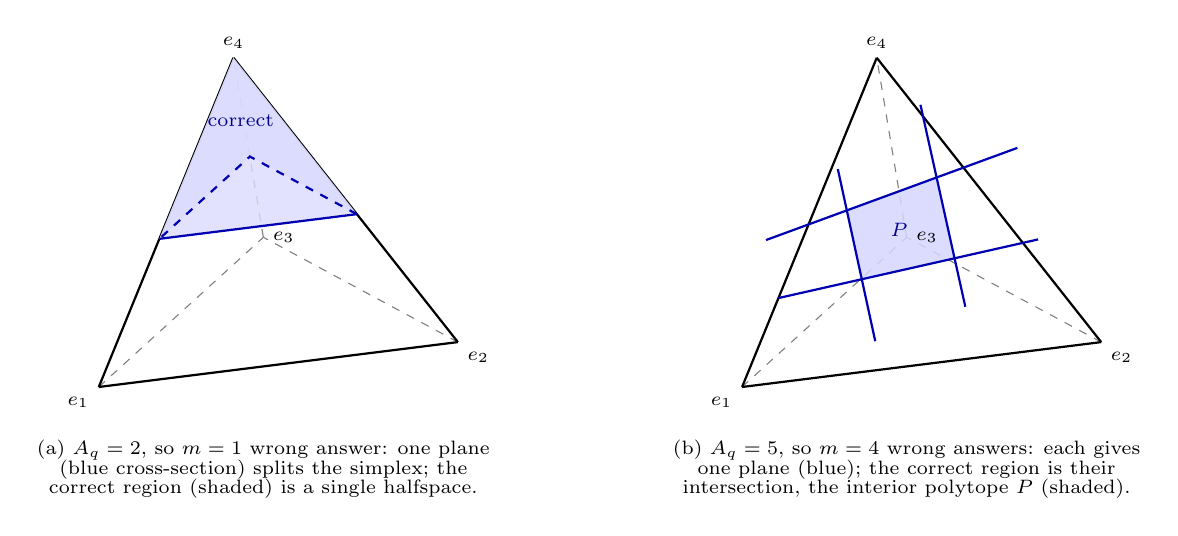
\begin{tikzpicture}[scale=1.9,
    every node/.style={font=\scriptsize}]
  % Panel (a): one wrong answer -> one halfspace
  \begin{scope}
    \coordinate (A) at (0,0);        % e_1
    \coordinate (B) at (2.4,0.3);    % e_2
    \coordinate (C) at (1.1,1.0);    % e_3 (back)
    \coordinate (D) at (0.9,2.2);    % e_4 (apex)
    % hidden edges to back vertex e_3
    \draw[gray,dashed] (A)--(C); \draw[gray,dashed] (B)--(C); \draw[gray,dashed] (C)--(D);
    % visible edges
    \draw[thick] (A)--(B) (A)--(D) (B)--(D);
    % cutting hyperplane {<w,delta>=0}: a triangular cross-section
    \coordinate (P1) at (0.405,0.99);   % on edge A--D
    \coordinate (P2) at (1.725,1.155);  % on edge B--D
    \coordinate (P3) at (1.01,1.54);    % on edge C--D
    % correct half (apex side) shaded
    \fill[blue!14,opacity=0.8] (P1)--(P2)--(D)--cycle;
    \fill[blue!14,opacity=0.8] (P1)--(P3)--(D)--cycle;
    \fill[blue!14,opacity=0.8] (P2)--(P3)--(D)--cycle;
    \draw[blue!70!black,thick] (P1)--(P2);
    \draw[blue!70!black,thick,dashed] (P2)--(P3)--(P1);
    \node[blue!55!black] at (0.95,1.78) {correct};
    \node[below left] at (A) {$e_1$};
    \node[below right] at (B) {$e_2$};
    \node[right] at (C) {$e_3$};
    \node[above] at (D) {$e_4$};
    \node[align=center] at (1.1,-0.55)
      {(a) $A_q=2$, so $m=1$ wrong answer: one plane\\[-1pt](blue cross-section) splits the simplex; the\\[-1pt]correct region (shaded) is a single halfspace.};
  \end{scope}
  % Panel (b): several wrong answers -> polytope
  \begin{scope}[xshift=4.3cm]
    \coordinate (A) at (0,0);
    \coordinate (B) at (2.4,0.3);
    \coordinate (C) at (1.1,1.0);
    \coordinate (D) at (0.9,2.2);
    \draw[gray,dashed] (A)--(C); \draw[gray,dashed] (B)--(C); \draw[gray,dashed] (C)--(D);
    \draw[thick] (A)--(B) (A)--(D) (B)--(D);
    % Four cutting planes; the shaded quadrilateral P below is EXACTLY the
    % intersection region, so each of its four edges lies on one blue line.
    \coordinate (Q1) at (0.80,0.72);
    \coordinate (Q2) at (1.42,0.86);
    \coordinate (Q3) at (1.30,1.40);
    \coordinate (Q4) at (0.70,1.18);
    % interior polytope P = intersection of the four halfspaces
    \fill[blue!16,opacity=0.85] (Q1)--(Q2)--(Q3)--(Q4)--cycle;
    % each blue line passes through two adjacent vertices of P and extends to the faces
    \draw[blue!70!black,thick] ($(Q1)!-0.9!(Q2)$)--($(Q2)!-0.9!(Q1)$); % edge Q1-Q2
    \draw[blue!70!black,thick] ($(Q2)!-0.6!(Q3)$)--($(Q3)!-0.9!(Q2)$); % edge Q2-Q3
    \draw[blue!70!black,thick] ($(Q3)!-0.9!(Q4)$)--($(Q4)!-0.9!(Q3)$); % edge Q3-Q4
    \draw[blue!70!black,thick] ($(Q4)!-0.6!(Q1)$)--($(Q1)!-0.9!(Q4)$); % edge Q4-Q1
    \node[blue!55!black] at (1.05,1.05) {$P$};
    \node[below left] at (A) {$e_1$};
    \node[below right] at (B) {$e_2$};
    \node[right] at (C) {$e_3$};
    \node[above] at (D) {$e_4$};
    \node[align=center] at (1.1,-0.55)
      {(b) $A_q=5$, so $m=4$ wrong answers: each gives\\[-1pt]one plane (blue); the correct region is their\\[-1pt]intersection, the interior polytope $P$ (shaded).};
  \end{scope}
\end{tikzpicture}
\caption{Correct-region of ensemble weights for a \emph{single} question $q$ with
$K=4$ models. The weight vector $w=(w_1,\dots,w_4)$ obeys $w_i\ge 0$ and
$w_1+w_2+w_3+w_4=1$, so it lives on the probability simplex; this constraint drops
one degree of freedom, turning the $4$-dimensional weights into a $3$-dimensional
solid \textbf{tetrahedron}. Its four \textbf{vertices} $e_1,\dots,e_4$ are the
pure weightings (vertex $e_i$ places all weight on model $i$); the black and
dashed lines are the tetrahedron's \emph{edges}, the boundary of the weight
domain.
Superimposed on this domain, each \textbf{blue line} is the trace of one decision
hyperplane $\{w:\ip{w}{\delta_{q,a}}=0\}$, one per wrong answer $a$, where the
ensemble is exactly tied with $a$, and the \textbf{shaded blue region} is the
correct-region $\{w:M_q(w)>0\}$, the weights that beat every wrong answer.
(a)~If the question has $A_q=2$ candidate answers there is $m=1$ wrong answer,
hence a single plane, and the correct-region is one halfspace (here $m$ blue
lines $=1$). (b)~If $A_q=5$ there are $m=4$ wrong answers, hence $4$ blue lines,
and the correct-region is the interior polytope $P$ where all four halfspaces
overlap.}
\label{fig:simplex}
\end{figure}
The maximum size of the answer set across questions is defined as
\begin{equation}
\label{eq:A}
A := \max_q |\Aq|.
\end{equation}

\subsection{A uniform-convergence baseline}
\label{sec:method-vc}

Fixing a problem, ``$M_q(w)\le 0$'' means $w$ lies outside an intersection of at
most $A-1$ homogeneous halfspaces in $\R^K$. A single halfspace-indicator class in
$\R^K$ has VC dimension $K$, and an intersection of $m$ of them has VC dimension
$O(Km\log m)$ by the Blumer composition bound \citep{blumer1989learnability}
(equivalently, the number of regions that $m$ hyperplanes cut $\R^K$ into is
polynomial in $m$, the classical hyperplane-arrangement count of
\citet{zaslavsky1975facing}). The \emph{capacity} of a hypothesis class is its VC
dimension, the largest number of problems the class can label in all possible
ways, a standard measure of how rich the class is and hence how much data uniform
convergence requires. Combining these gives
\begin{equation}
\label{eq:vc}
\VC(\Fcal) = \Too(KA),
\end{equation}
where $\Too(\cdot)$ is the usual $O(\cdot)$ up to logarithmic factors (here in $A$
and $Q$), which we suppress for readability. This yields the standard
uniform-convergence guarantee, our baseline.

\begin{theorem}[Uniform convergence over problems, \solid]%
\footnote{This theorem is fully proved in Appendix~\ref{app:proofs-gen}, as
opposed to results below that are stated with proof sketches or posed as open;
see the discussion of proof status in Section~\ref{sec:intro}.}
\label{thm:convergence}
There is a universal constant $c>0$ such that, with probability at least
$1-\delta$ over the $Q$ i.i.d.\ problems, simultaneously for all $w\in\simplex$,
\begin{equation}
\label{eq:thm1}
\big|\Risk(w)-\eRisk(w)\big|
\;\le\;
c\sqrt{\frac{KA\log A\,\log Q + \log(1/\delta)}{Q}}.
\end{equation}
\end{theorem}

\begin{proof}[Proof sketch]
Standard VC/Rademacher symmetrization with Sauer's lemma
\citep{sauer1972density,shelah1972combinatorial,vapnik1971uniform} applied to
$\Fcal$, using the capacity \eqref{eq:vc}. The $\log A$ and $\log Q$ factors are
the logarithmic overheads incurred when bounding the VC dimension of an
intersection of $A-1$ halfspaces (the $\log A$) and when passing from the growth
function to a uniform bound over $Q$ problems (the $\log Q$); these are exactly
the logarithmic terms absorbed into $\Too(\cdot)$ in \eqref{eq:vc}. Full argument
in Appendix~\ref{app:proofs-uc}.
\end{proof}

Inverting \eqref{eq:thm1} gives the sample-complexity reading
\begin{equation}
\label{eq:qneed}
Q \gtrsim \frac{KA}{\epsilon^2}\quad\text{for a gap}\le\epsilon,
\end{equation}
which is loose but correctly predicts the $1/\sqrt Q$ decay across benchmarks.
We record a PAC-Bayes tightening as an optional remark, not a headline
contribution; converting its randomized (Gibbs) guarantee to the deployed
deterministic weights relies on C-bound / Chebyshev--Cantelli arguments
\citep{viallard2021selfboundingmv,wu2021chebyshevcantellipi}.

% \begin{remark}[PAC-Bayes, demoted]
% \label{rem:pacbayes}
% Replacing the class-wide capacity by the divergence of a data-chosen posterior
% $\Qcal$ from a prior $\Pcal$ gives the McAllester bound on the Gibbs risk
% \citep{mcallester1999pacbayes},
% \begin{equation}
% \label{eq:mcallester}
% \E_{w\sim\Qcal}\Risk(w)
% \le
% \E_{w\sim\Qcal}\eRisk(w)
% + \sqrt{\frac{\KL(\Qcal\|\Pcal) + \log(2\sqrt Q/\delta)}{2(Q-1)}},
% \end{equation}
% minimized (for fixed $\Pcal$, $\lambda>0$) by the Gibbs posterior
% \begin{equation}
% \label{eq:gibbs}
% \Qcal^\star(w)\propto \Pcal(w)\,e^{-\lambda\eRisk(w)}.
% \end{equation}

% Two caveats keep this off the critical path: converting the Gibbs risk to the
% deployed deterministic $w$ costs a factor via C-bound/Chebyshev--Cantelli
% arguments \citep{viallard2021selfboundingmv,wu2021chebyshevcantellipi}, and a
% uniform posterior with $\KL(\Qcal\|\text{uniform})=0$ can certify a comparable
% bound, so a favorable number may reflect the class rather than the learner. We
% treat \eqref{eq:mcallester} as an appendix ablation.
% \end{remark}

\subsection{Decomposing the excess risk into a $Q$-term and an $N$-term}
\label{sec:method-decomp}

Let $\wstar$ be the best population weights and $\what$ the weights returned by
fitting the empirical margins (the Komiyama MILP \citep{komiyama2026best}, or any
surrogate),
\begin{equation}
\label{eq:wstar-what}
\wstar = \argmin_{w\in\simplex}\Risk(w),
\qquad
\what \in \argmin_{w\in\simplex}\eRisk(w).
\end{equation}
The weight-learning procedure in \eqref{eq:wstar-what} can only see empirical
margins, so the risk it can actually target lives at the empirical-margin level.
We define the empirical-margin risk, an expectation over both the problem draw
and the $N$ generations,
\begin{equation}
\label{eq:RN}
\Risk_N(w) := \Pr_{q,\,\text{gen}}\!\big[\Mhat_q(w)\le 0\big].
\end{equation}
The excess risk then splits into three pieces that isolate the two sample sizes,
\begin{equation}
\label{eq:decomp}
\Risk(\what) - \Risk(\wstar)
=
\underbrace{\big[\Risk(\what) - \Risk_N(\what)\big]}_{\text{(i) margin estimation, }N}
+ \underbrace{\big[\Risk_N(\what) - \Risk_N(\wstar)\big]}_{\text{(ii) problem sampling, }Q}
+ \underbrace{\big[\Risk_N(\wstar) - \Risk(\wstar)\big]}_{\text{(iii) margin estimation, }N}.
\end{equation}
Terms (i) and (iii) depend on the estimation noise from the $N$ generations, so
we group them as the \emph{$N$-term} (the error term driven by margin
estimation); term (ii) depends on the problem sample and is the \emph{$Q$-term}
(driven by problem sampling). This single identity is central to the paper:
everything below bounds these two terms and ties both to one exponent.

\paragraph{Worked example.}
Take $K=2$, $Q=3$ problems, weights $\wstar$, and true margins
$M_1(\wstar)=0.30,\ M_2(\wstar)=0.02,\ M_3(\wstar)=-0.25$, so $\Risk(\wstar)=1/3$
(problem $3$ wrong). At small $N$ the near-tie problem $q=2$ ($M_2=0.02$) can flip
sign in $\Mhat$; if it flips, $\Risk_N(\wstar)=2/3$, contributing $+1/3$ to term
(iii). The well-separated problems $q=1,3$ almost never flip. The gap between
$\Risk_N$ and $\Risk$ is thus driven entirely by mass near zero, the $N$-floor.

\subsection{The margin exponent and the two rates}
\label{sec:method-rates}

The baseline bound \eqref{eq:thm1} decays at the slow $1/\sqrt Q$ rate, which
holds for \emph{any} problem distribution and is therefore pessimistic: it
ignores that on most benchmarks the ensemble is not borderline on a typical
problem, but wins (or loses) by a comfortable margin. The problems that are
genuinely hard, for both learning the weights and estimating the margins from
$N$ generations, are the near-ties, those whose true margin $M_q(\wstar)$ sits
close to zero, because a small perturbation can flip them from correct to wrong.
Intuitively, then, the difficulty of the problem is controlled by \emph{how much
of the problem mass concentrates near the decision boundary} $M_q(\wstar)=0$. The
margin (Tsybakov) exponent $\beta$ makes this precise: a larger $\beta$ means
fewer near-tie problems, which we will show both accelerates the $Q$-term beyond
$1/\sqrt Q$ and sets the size of the irreducible $N$-floor. This is the source of
our faster, distribution-dependent rates below.

In the following, $\wstar$ is a fixed (deterministic) vector, the optimal weights
of \eqref{eq:wstar-what}, while the problem $q\sim\D$ is random; hence
$M_q(\wstar)$ is a scalar random variable, one real number per problem (its value
is the smallest of the $m=A_q-1$ gaps against the wrong answers). The probability
below is taken over the random draw of $q$.
\begin{definition}[Margin exponent $\beta$]
\label{def:tsybakov}
The problem distribution $\D$ has margin exponent $\beta\ge 0$ if there is a
constant $C>0$ with
\begin{equation}
\label{eq:margincond}
\Pr_{q\sim\D}\!\big[\,0 < |M_q(\wstar)| \le t\,\big] \le C\,t^{\beta}
\qquad \forall t>0.
\end{equation}
\end{definition}

\paragraph{Example.}
If the true margins $M_q(\wstar)$ are uniform on $[-1,1]$, then
$\Pr[|M_q|\le t] = t$, so $\beta=1$. If all margins are bounded away from zero,
say $|M_q(\wstar)|\ge m_0>0$ a.s., then \eqref{eq:margincond} holds for all
$\beta$, i.e.\ $\beta=\infty$: no near-ties, and both terms vanish fastest.

The $Q$-term is classical excess risk for the frozen loss over $\Fcal$; the
margin condition accelerates it in the Mammen--Tsybakov manner
\citep{mammen1999smooth,tsybakov2004optimal}.

\begin{proposition}[Accelerated $Q$-rate]
\label{prop:1}
Under \eqref{eq:margincond} with exponent $\beta$, the $Q$-term of
\eqref{eq:decomp} obeys
\begin{equation}
\label{eq:qrate}
\text{\emph{(ii)}} \;=\; \Too\!\left(\Big(\frac{KA}{Q}\Big)^{\frac{\beta+1}{\beta+2}}\right),
\end{equation}
interpolating between the slow rate $\sqrt{KA/Q}$ at $\beta=0$ and the fast rate
$KA/Q$ as $\beta\to\infty$.
\end{proposition}

\noindent This is a transport of Tsybakov's local-Rademacher/peeling framework
\citep{bartlett2005local,koltchinskii2006local,massart2006risk} to the class
$\Fcal$; the full argument is given in Appendix~\ref{app:proofs-gen}. Two
features of our setting make it non-standard.
First, recall that the ensemble predicts by $f_w(q)=\argmax_a S_w(a\mid q)$ with
the mixture score $S_w(a\mid q)=\sum_i w_i\,p_i(a\mid q)$ of
\eqref{eq:score}. The key observation is that the gap of a wrong answer $a$
is exactly the score of the gold answer $a_q^\star$ minus the score of $a$,
\begin{equation}
\label{eq:gap-is-score-diff}
\ip{w}{\delta_{q,a}}
= \sum_i w_i\big(p_i(a_q^\star\mid q)-p_i(a\mid q)\big)
= S_w(a_q^\star\mid q) - S_w(a\mid q),
\end{equation}
which is why we take the gap over wrong answers $a\ne a_q^\star$ only: it measures
how far $a_q^\star$'s score $S_w(a_q^\star\mid q)$ is \emph{above} the score
$S_w(a\mid q)$ of each competing answer, and comparing $a_q^\star$ with itself
gives the trivial gap $0$, so it is excluded. The ensemble's predicted answer is
the one with the highest score, $f_w(q)=\argmax_{a\in\Aq} S_w(a\mid q)$; we say
$a_q^\star$ ``wins'' when it is this $\argmax$, i.e.\ when the ensemble predicts
$a_q^\star$ and is therefore correct. By \eqref{eq:gap-is-score-diff}, $a_q^\star$
attains the highest score iff its score exceeds that of every wrong answer, i.e.\
iff every gap in \eqref{eq:gap-is-score-diff} is positive, i.e.\ iff
$M_q(w)=\min_{a\ne a_q^\star}\ip{w}{\delta_{q,a}}>0$. This is why $M_q(w)>0$ is
exactly the condition for a correct answer. The answer $a_q^\star$ does \emph{not}
automatically attain the highest score: if some wrong answer $a$ has
$S_w(a\mid q)>S_w(a_q^\star\mid q)$, then
$S_w(a_q^\star\mid q)-S_w(a\mid q)<0$, so that gap is negative and $M_q(w)<0$
(the ensemble predicts $a$ and is wrong). Because correctness requires beating \emph{all}
contenders at once, the margin is set by the single hardest one, the contender
with the smallest gap. Consequently the
Tsybakov low-noise condition, which in the standard binary-classification setting
concerns behavior near one decision boundary (the single surface where the
classifier switches its label), must here be checked against this worst contender
at every $w$ rather than against one fixed boundary.
Second, $\what$ is fit on the noisy empirical margins, i.e.\ it minimizes
$\Risk_N$ (defined in \eqref{eq:RN}) rather than the population risk $\Risk$.
Recall that each model's answer distribution $\phat_i(\cdot\mid q)$ is estimated
from its $N$ sampled outputs on problem $q$, so both the objective $\Risk_N$ that
selects $\what$ and the empirical margins used to bound the risk are computed from
the \emph{same} $N$ samples. Because the same
random draws feed both, the $Q$-term (problem sampling) and the $N$-term (margin
estimation) are statistically dependent rather than independent, so we cannot
bound them separately and add; the proof must control their interaction.

We now bound the $N$-term. Each empirical margin $\Mhat_q(w)$ is an average over
the $N$ generations, so it estimates the true margin $M_q(w)$ to accuracy of
order $1/\sqrt N$ (the standard deviation of an $N$-sample mean). The ensemble's
answer on problem $q$ is decided by the \emph{sign} of the margin: recall from
\eqref{eq:M} that $M_q(w)=\min_{a\ne a_q^\star}\ip{w}{\delta_{q,a}}$ is the
mixture's gap to its hardest wrong answer, so $M_q(w)>0$ means the mixture scores
the gold answer above every wrong answer (the prediction $f_w(q)$ is correct),
while $M_q(w)<0$ means some wrong answer outscores the gold answer (incorrect).
The verdict therefore changes only if the estimation error
\begin{equation}
\label{eq:margin-error}
\eps_q(w) := \Mhat_q(w) -q M_q(w), \qquad |\eps_q(w)| = O(1/\sqrt N),
\end{equation}
is large enough to push the estimated margin $\Mhat_q(w)=M_q(w)+\eps_q(w)$ across
zero, i.e.\ to make $\Mhat_q(w)$ and $M_q(w)$ have opposite signs. This can happen
only when the \emph{true} margin is itself within about $1/\sqrt N$ of zero: if
$|M_q(w)|\gg 1/\sqrt N$, then $\Mhat_q(w)=M_q(w)+\eps_q(w)$ keeps the sign of
$M_q(w)$ because $|\eps_q(w)|=O(1/\sqrt N)<|M_q(w)|$. In words, only problems
whose true margin is a near-tie (within an $O(1/\sqrt N)$-wide interval around
$0$) are at risk of being misclassified because of sampling noise; well-separated
problems are essentially never flipped. The next lemma makes this precise.

\begin{lemma}[Margin sign reliability, \solid]
\label{lem:1}
Fix $w\in\simplex$ and problem $q$. Each estimate $\phat_i(a\mid q)$ is the
fraction of the $N$ generations of model $i$ that return answer $a$, i.e.\ a mean
of $N$ i.i.d.\ Bernoulli draws, so each coordinate of the empirical gap
$\dhat_{q,a}$ is a difference of two such means,
\begin{equation}
\label{eq:bern}
(\dhat_{q,a})_i = \phat_i(a_q^\star\mid q) - \phat_i(a\mid q),
\qquad
\phat_i(a\mid q) = \frac1N\sum_{n=1}^N \mathbf 1[\text{generation }n\text{ is }a].
\end{equation}
Since a mean of $N$ bounded variables has variance $O(1/N)$, the empirical margin
has variance
\begin{equation}
\label{eq:var}
\mathrm{Var}\big(\Mhat_q(w)\big) \;\le\; \frac{c\,\|w\|_2^2}{N} \;\le\; \frac{c}{N}.
\end{equation}
Consequently, for a problem with true margin $|M_q(w)| = m$, a Hoeffding/Bernstein
bound \citep{hoeffding1963probability} and a union over at most $A-1$ contenders
bound the probability that the estimated margin has a \emph{different sign} than
the true margin (i.e.\ the ensemble's correct/incorrect verdict flips relative to
the truth) by
\begin{equation}
\label{eq:signflip}
\Pr\!\big[\sign(\Mhat_q(w)) \ne \sign(M_q(w))\big]
\;\le\; (A-1)\,\exp\!\big(-c\,N\,m^2\big),
\end{equation}
where $\sign(\cdot)$ records only whether its argument is positive or negative,
so $\sign(\Mhat_q)\ne\sign(M_q)$ is exactly the event that estimation noise turns
a truly-correct problem into a predicted-wrong one, or vice versa.
\end{lemma}

\noindent Let us unpack \eqref{eq:signflip}. The ensemble's prediction on
problem $q$ is correct exactly when $M_q(w)>0$ (the mixture's top-scoring answer
is the gold one), so the only thing that matters for accuracy is the \emph{sign}
of the margin. There are two signs available: the sign of the true margin
$M_q(w)$, which gives the correct answer, and the sign of the empirical margin
$\Mhat_q(w)$, which is what we actually compute from the $N$ samples. A problem is
misclassified precisely when these two disagree, i.e.\ the sign-flip event
$\sign(\Mhat_q(w))\ne\sign(M_q(w))$, and \eqref{eq:signflip} bounds its
probability by $(A-1)\exp(-c\,N\,m^2)$, where $m=|M_q(w)|$ is the size of the true
margin. This bound has two regimes. When $M_q(w)$ is well clear of a tie,
$m\gg 1/\sqrt N$, the exponential is tiny and a flip almost never happens; when
$M_q(w)$ is a near-tie, $m\lesssim 1/\sqrt N$, the estimation error $\eps_q(w)$
is comparable to $M_q(w)$ itself and $\sign(\Mhat_q(w))$ is close to a coin flip.
Consequently the only problems that contribute error from finite sampling are
those whose true margin lies in the narrow interval $|M_q(w)|\lesssim 1/\sqrt N$
around zero. This is why the sign-flip event is the quantity we track: it
isolates the finite-$N$ error to the mass of near-tie problems. Proposition~\ref{prop:2}
below bounds the $N$-term by this near-tie mass, $\Pr_q[\,|M_q(\wstar)|\le c/\sqrt N\,]$,
which involves $N$ but not $Q$: it stays the same however many problems we
collect, because a near-tie problem flips whenever its own $N$ generations are
too few to resolve $\sign(M_q)$, and adding \emph{other} problems does nothing to
sharpen that one problem's margin estimate.

\begin{proposition}[The $N$-floor]
\label{prop:2}
Under \eqref{eq:margincond}, the total $N$-term contribution of
\eqref{eq:decomp} satisfies
\begin{equation}
\label{eq:floor}
\big|\text{\emph{(i)}} + \text{\emph{(iii)}}\big|
\;\lesssim\;
\Pr_q\!\Big[\,|M_q(\wstar)|\le \tfrac{c}{\sqrt N}\,\Big]
\;\overset{\eqref{eq:margincond}}{\le}\;
C\Big(\tfrac{c}{\sqrt N}\Big)^{\beta}
\;=\; O\!\big(N^{-\beta/2}\big).
\end{equation}
\end{proposition}

\noindent The proof is given in Appendix~\ref{app:proofs-gen}. Recall from the
decomposition \eqref{eq:decomp} that the excess risk splits into three terms:
term (ii) is the $Q$-term, driven by problem sampling, while terms (i) and (iii)
are the two $N$-terms, driven by margin-estimation noise. Proposition~\ref{prop:2}
bounds only the $N$-terms (i)$+$(iii); the $Q$-term (ii) is handled separately by
the accelerated $Q$-rate of Proposition~\ref{prop:1}, which is why it does not
appear here. We call the
bound $O(N^{-\beta/2})$ in \eqref{eq:floor} the \emph{$N$-floor} because it is a
lower limit on the $N$-terms that depends only on $N$ and $\beta$ and is
\emph{completely independent of $Q$}: increasing the number of problems $Q$
drives the $Q$-term to zero but leaves the $N$-terms untouched, since they are
caused by near-tie problems ($|M_q(\wstar)|\lesssim 1/\sqrt N$) whose margins the
finite $N$ generations cannot estimate accurately e5nough to recover $\sign(M_q)$,
however many problems we collect. Here $1/\sqrt N$ is the accuracy of the
empirical margin: it is the size of the estimation error $\eps_q(w)$ from
\eqref{eq:margin-error}, so a margin closer to zero than $1/\sqrt N$ cannot be
distinguished from a tie. Term (iii) follows directly from Lemma~\ref{lem:1} and
\eqref{eq:margincond}; term (i) additionally requires a uniform-over-$w$ version
of Lemma~\ref{lem:1}, a Rademacher bound on the process
$\{\Mhat_q(\cdot)-M_q(\cdot)\}$ indexed by $w\in\simplex$, which is sub-Gaussian
with a $K$-dimensional index and controls the winner's-curse bias at scale
$\sqrt{K/N}$. Making the constant in this $\sqrt{K/N}$ bound explicit is the one
step of this argument we leave to future work; we state term (i) with a proof
sketch and flag it accordingly in Section~\ref{sec:theory}.

Assembling the two terms through the triangle inequality on
\eqref{eq:decomp} gives the central result.

\begin{theorem}[Joint $(N,Q)$ excess risk, \conjecture]
\label{thm:main}
Under the margin condition \eqref{eq:margincond} with exponent $\beta$,
\begin{equation}
\label{eq:joint}
\boxed{\;
\Risk(\what) - \Risk(\wstar)
\;\lesssim\;
\underbrace{\Big(\tfrac{KA}{Q}\Big)^{\frac{\beta+1}{\beta+2}}}_{\text{collect more problems}}
\;+\;
\underbrace{C\,N^{-\beta/2}}_{\text{sample each model more}}
\;}
\end{equation}
\end{theorem}


\section{Experiments}
\label{sec:experiments}



\appendix


\bibliographystyle{iclr2026_conference}
\bibliography{iclr2026_conference}

\end{document}
